\documentclass{article}
\usepackage{graphicx}
\usepackage{lmodern} % Fix the font size warnings
\usepackage{fancyhdr} % Required for custom headers
\usepackage{lastpage} % Required to determine the last page for the footer
\usepackage{extramarks} % Required for headers and footers
\usepackage{graphicx} % Required to insert images
\usepackage{xfrac} % Nice fractions
\usepackage{amsmath}

\usepackage{multicol}

% Margins
\topmargin=-0.5in
\evensidemargin=0in
\oddsidemargin=-0.5in
\textwidth=7.5in
\textheight=9.0in
\headsep=0.25in 

% paragraphs
\usepackage{parskip}

\pagestyle{fancy}

\rhead{Main courses} % Top right header
\lhead{\textbf{Mom's Meatballs}}
\chead{}
\title{Mom's Meatballs}

\begin{document}
This sorta, kinda, started as Nana's meatballs recipe and she would make it every time Caitlyn
when to their house in Redmond. Well, mom took that recipe, made a few changes and made it her
own. Of the two Miller meatball recipes, this is Caitlyn's favorite.

\textbf{Meatballs}

\begin{itemize}
      \item 2 16 ounce packages of ground turkey (93\% Lean)
      \item 1 piece of bread
      \item 1 egg
      \item 1 large clove of crushed garlic
      \item 1\sfrac{1}{2} tsp of oregano
\end{itemize}

To prepare the meatballs shred the bread into tiny pieces and put in food processor with the egg, oregano, and garlic.
Blend this first until well mixed. Then add one package of turkey, process until combined and then add the other package.
Once meatball mix is done use a medium sized cookie scoop to form your meatballs.

\textbf{Sauce}

\begin{itemize}
      \item 3 cans of 32oz crushed tomatoes
      \item 1 medium shallot (chopped fine)
      \item 3 cloves of garlic (sliced thin)
      \item 3 tablespoons of olive oil
      \item 1 tsp of basil
      \item 1 tsp of oregano
      \item 1 tsp of parsley
\end{itemize}

To prepare the sauce sauté the onions and garlic in olive oil until translucent. Be careful because you don't want to burn
them. Add the 3 cans of crushed tomatoes, basil, oregano, and parsley and stir until combined. Let this simmer for about 30
minutes.

\textbf{Putting it all together}

Add the meatballs to the sauce one a time and cook for at least 1\sfrac{1}{2} hours. Stir every 15 minutes or so to make
sure that the sauce doesn't burn and that the meatballs get well cooked. You can check the meatballs are done using
an instant read thermometer inserted into the middle of a meatball. They are ``done'' when the temperature reaches
165 degrees. It's ok to cook them longer.


% \begin{figure}
%     \centering
%     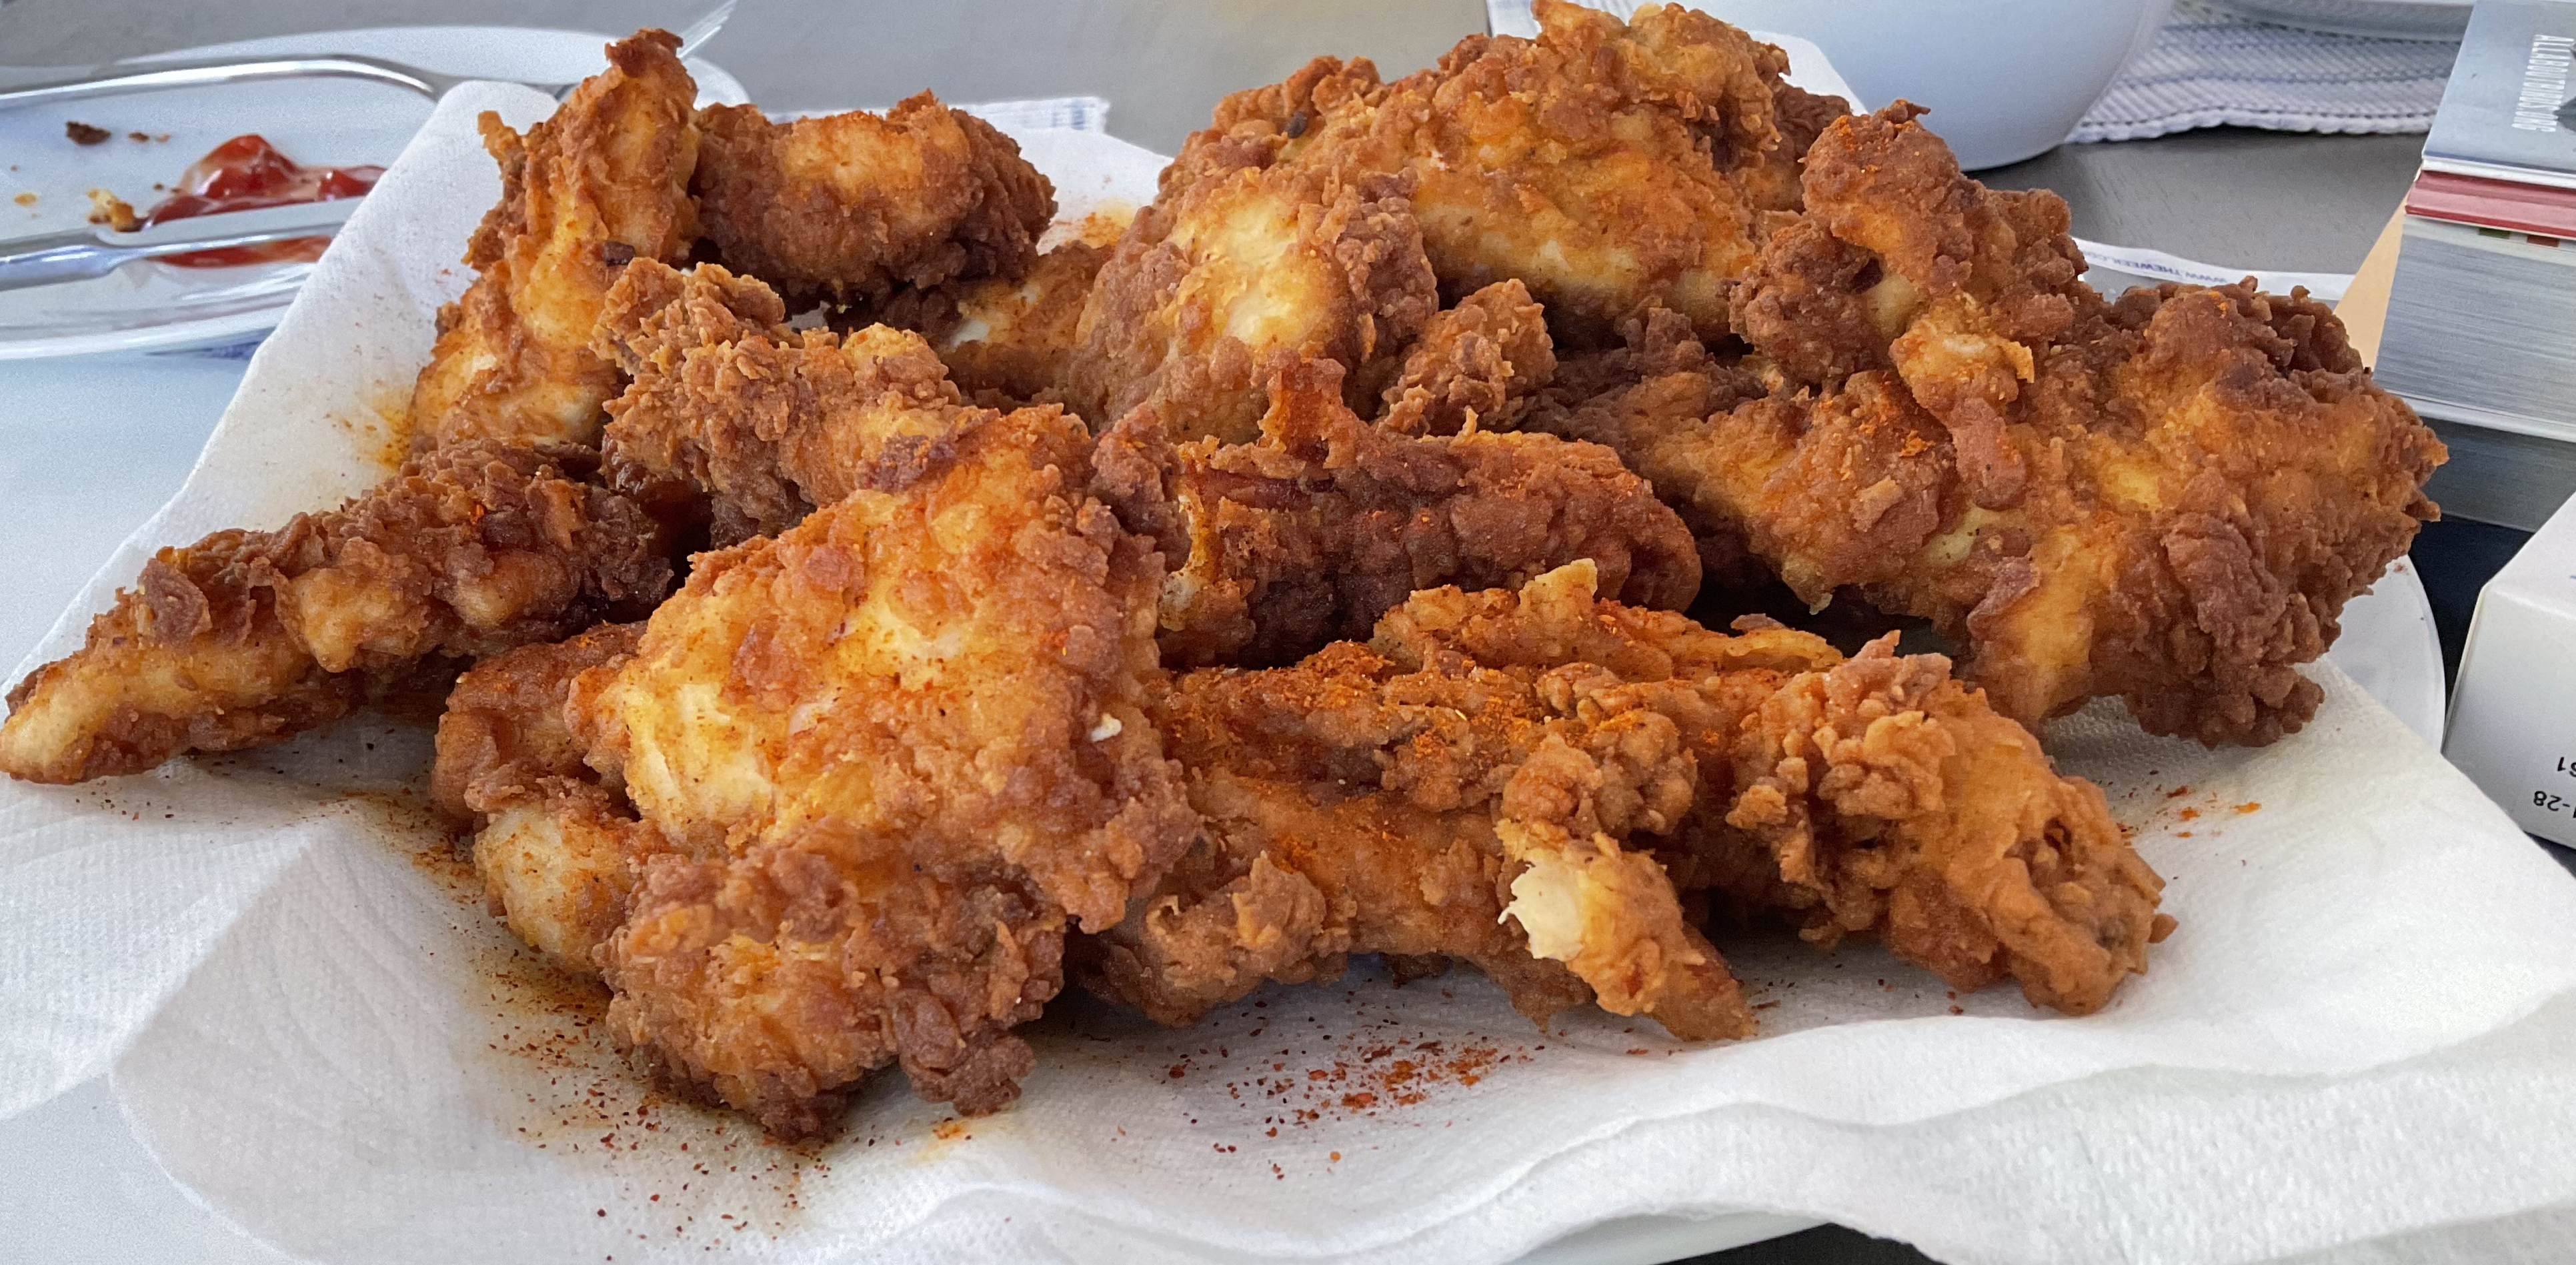
\includegraphics[scale=0.095]{fried-chicken.png}
% \end{figure}

\end{document}
